\section{Day-ahead capacity commitment on the U.S.\ grid}\label{sec:app}

\subsection{Data}

We use the complete public record of the U.S.\ Energy Information Administration's Hourly Electric Grid Monitor (Form EIA-930; \citealp{EIA930}), downloaded on 29 September 2026.
For every balancing authority (BA) in the lower 48 states the file reports hourly demand, the BA's own day-ahead demand forecast and total interchange with neighbouring BAs.
We use the period 1 January 2019 to 26 September 2026 in UTC hours and exclude the fourteen regional aggregates.
Following \citet{Ruggles2020}, non-positive values and values outside $[0.3,3]$ times the median of the preceding seven days are treated as missing, and gaps of up to three hours are interpolated; the filter is one-sided, so it uses no future data, and the official forecast is filtered against its own history rather than against realised demand.
We keep BAs with at least 97\% valid demand, at least 93\% valid official forecasts, mean demand above 50\,MW and a median absolute official forecast error below 15\% of median demand.
Forty-six BAs remain (Table~\ref{tab:bas} in Appendix~\ref{app:data}); they range from PJM (mean demand 92.5\,GW) to the City of Homestead (71\,MW), include all seven independent system operators, and account for 97\% of lower-48 demand.
Ten BAs are dropped, mostly small systems with long gaps or implausible official forecasts; 0.27\% of the retained BA-hours are missing.

\subsection{Decision problem and cost calibration}

On the morning of day $d-1$, before the day-ahead gate closure, BA $i$ commits hourly capacity $q_{i,d,h}$, $h=0,\dots,23$, for the (UTC) operating day $d$.
At that time demand is observed only up to the end of day $d-2$: the UTC day $d-1$ ends in the afternoon or evening of local day $d-1$ in the United States, after any day-ahead deadline.
The information set therefore contains realised demand up to the end of day $d-2$, the realised costs of every rule up to the same day, and the BA's published day-ahead forecast for day $d$; every candidate, margin and estimation window below respects this timing.
This is a conservative convention: an operator could also use the hours of day $d-1$ observed before the gate closure, which would favour the data-driven candidates slightly.
Excess commitment costs $o_i=1$ per MWh, which normalises all costs to units of the per-MWh cost of idle committed capacity.
Shortfalls cost $u_i=\tau_i/(1-\tau_i)$, where the critical ratio $\tau_i$ is meant to reflect how easily the BA can lean on its neighbours.
As a transparent proxy we use the variability of interchange in the pre-sample year 2019---the range between the 5th and 95th percentiles of hourly total interchange, divided by mean demand---and let $\tau_i$ decline linearly in its rank from $0.95$ for the BA with the least variable interchange to $0.80$ for the one with the most.
Interchange variability is not transfer capability, and shortfall costs in practice depend on market prices and system conditions; the proxy only orders BAs plausibly, and Section~\ref{sec:robust} reports the results under common critical ratios from 0.5 to 0.95 (and Section~\ref{sec:global} for the global panel under a scarcity-level ratio of 0.99).
ERCOT, which is almost islanded, receives $\tau=0.95$ ($u_i=19$); the Chelan County PUD in the densely interconnected Pacific Northwest receives $\tau=0.80$ ($u_i=4$).

\subsection{Candidate rules}

Seven candidate forecasts are produced for every BA, day and hour, each using only the information available at the decision time:
(1) the BA's official day-ahead forecast;
(2) persistence (same hour of $d-2$);
(3) weekly persistence (same hour of $d-7$);
(4) the mean of the same hour over $d-2,\dots,d-8$;
(5) the mean of the same hour on $d-7$, $d-14$ and $d-21$;
(6) a BA-and-hour-specific linear regression on the $d-2$ and $d-7$ values, the official forecast and weekday dummies, estimated on a rolling 56-day window and refitted weekly; and
(7) a single global LightGBM model \citep{Ke2017} across all BAs and hours, trained on lags, calendar variables and the official forecast, all scaled by the BA's recent mean demand, refitted every 28 days on the preceding 365 days.
Every training window ends at day $d_0-2$ for forecasts made at origin $d_0$.
Model (7) is the kind of machine-learning forecaster a central planner could run for every BA at low cost.
Each forecast $f^{(m)}$ becomes a candidate commitment by adding its own safety margin,
\[
q^{(m)}_{i,d,h}=f^{(m)}_{i,d,h}\,\big\{1+\widehat Q_{\tau_i}(e^{(m)}_i)\big\},
\]
where $\widehat Q_{\tau_i}(e^{(m)}_i)$ is the empirical $\tau_i$-quantile of the relative errors $(y-f^{(m)})/\max\{f^{(m)},0.2\bar y_{i,t}\}$ of forecast $m$ for BA $i$ over the 28 days ending at $d-2$; the floor at 20\% of the BA's mean demand $\bar y_{i,t}$ over the week before the error's day $t$ prevents an occasional implausibly small forecast from producing an unbounded margin.
The candidate rules are available from February 2020, so the evaluation period runs from 1 April 2020 to 26 September 2026: 2,342 days, 335 weekly re-estimations and 2.58 billion MWh of demand.

\subsection{Competing methods}

Every seven days, at origin $d_0$, each method re-estimates its combination from the $W$ most recent days whose outcomes are known, $d_0-W-1,\dots,d_0-2$, $W\in\{7,14,28,56\}$ (each day contributes 24 hourly observations per BA), and commits for the following seven days.
Besides GDMA and soft GDMA ($G_{\max}=6$) we consider:
the official-forecast policy (candidate~1 alone), the reference rule in the U.S.\ analysis---a stylised version of committing on the operator's own forecast, since actual commitment runs through market clearing, reliability unit commitment and reserve procurement;
equal weights over the seven candidates;
the best single candidate per BA over the window;
pooled decision-focused weights;
per-BA decision-focused weights (the decision-focused analogue of per-series forward validation);
shrinkage of per-BA weights towards pooled weights with the shrinkage intensity chosen on the hold-out (a decision-focused version of \citealp{DieboldShin2019});
two-step clustering, which runs $k$-means on the per-BA weight vectors and re-estimates pooled weights within clusters, with the number of clusters chosen by the same hold-out and one-standard-error rule as GDMA;
a linear quantile-regression combination, which regresses demand on the seven point forecasts at each BA's critical ratio $\tau_i$ without the simplex constraint (the natural decision-focused combination of \citealp{Wang2019cqra});
and two \emph{forecast-then-commit} methods, which estimate per-BA or grouped combination weights by minimising scaled squared forecast error and then add the $\tau_i$-quantile of the combined forecast's relative errors over the same 28 days that set the candidates' margins.
The last two isolate the value of estimating the combination for the decision rather than for accuracy.
All hold-out choices ($G$, $\kappa$ and the shrinkage intensity) use the same split of the estimation window: every third day, counted back from the end of the window, is a validation day, so that the validation days span the window and cycle through the days of the week across origins.

\subsection{Results}

\begin{table}[t]
\centering
\caption{Out-of-sample system-wide commitment cost, 1 April 2020 to 26 September 2026, relative to committing on the official day-ahead forecasts. $W$ is the length of the estimation window. Bold: lowest cost in the column. Stars: Diebold--Mariano test of equal daily system cost against soft GDMA with Newey--West variance (7 lags); $^{*}$, $^{**}$, $^{***}$: $p<0.10,0.05,0.01$.}\label{tab:main}
\footnotesize
\begin{tabular}{@{}lcc@{}}
\toprule
 & \multicolumn{1}{c}{System cost relative to the official-forecast policy} & \\
\cmidrule(lr){2-2}
Method & $W=7$ & Share of BAs \\
 & days & improved$^a$ \\
\midrule
Official forecast & 1.0000$^{***}$ & 0.00 \\
Equal weights & 1.5322$^{***}$ & 0.13 \\
Best single (per BA) & 0.8490$^{***}$ & 0.59 \\
Pooled DF weights & 0.8156 & 0.72 \\
Per-BA DF weights & 0.8497$^{***}$ & 0.57 \\
Shrinkage to pooled & \textbf{0.8154} & 0.72 \\
Two-step $k$-means & 0.8243 & 0.70 \\
Forecast-then-commit, per BA & 0.9713$^{***}$ & 0.46 \\
Forecast-then-commit, grouped & 0.9068$^{***}$ & 0.57 \\
\textbf{GDMA} & 0.8163 & 0.72 \\
\bottomrule
\end{tabular}
\par\smallskip\footnotesize $^a$ Share of the 46 BAs whose own cost is lower than under the official-forecast policy ($W=28$).
\end{table}

Table~\ref{tab:main} contains the main result.
Four findings stand out.

\emph{First, deciding for the decision pays.}
Soft GDMA lowers the system-wide commitment cost by 18--20\% relative to the status quo of committing on the official forecasts, and every decision-focused combination method lowers it by at least 15\%; all reductions are significant at the 1\% level.
The forecast-then-commit methods, which combine the same seven forecasts for accuracy and then add a quantile margin, save only 3--18\%, and they are significantly more expensive than soft GDMA for every window length.
The gap is largest when windows are short ($W=7$: 0.971 and 0.907 against 0.817), because accuracy-optimal weights are chosen without regard to the asymmetric costs and the margin estimated from one week of combined errors is noisy.
Equal weights are the worst choice: they give weight to the naive calendar rules and raise cost by 53\%.

\emph{Second, neither extreme is right.}
Per-BA weights are expensive when windows are short (0.850 at $W=7$, 4.2\% above pooled weights), pooled weights are expensive when windows are long (0.804 at $W=56$, 0.9\% above soft GDMA), and the per-window ranking of the two reverses between $W=14$ and $W=28$.
This is the bias--variance trade-off of Theorem~\ref{thm:oracle} in action.

\emph{Third, soft GDMA is the most reliable method.}
It has the lowest system cost for $W=14$ and $W=28$ and is within 0.1\% of the best method for $W=7$ and $W=56$; no method is significantly cheaper than soft GDMA for any window, while it is significantly cheaper than pooled weights, per-BA weights, the forecast-then-commit methods and plain GDMA for most windows.
Its closest competitor is decision-focused shrinkage towards pooled weights, which is the special case $G=1$ of soft GDMA and is statistically indistinguishable from it; the two coincide exactly in the 57--68\% of weeks (depending on $W$) in which the hold-out rule selects a single segment.
Plain GDMA improves significantly on pooled weights for $W\ge14$ and on per-BA weights for $W\le14$, but forcing all members of a segment onto identical weights costs 0.4--0.5\% relative to soft segments when $W\ge14$.
Choosing $G$ by the plain hold-out minimum instead of the one-standard-error rule is worse for short windows (0.823 against 0.816 at $W=7$), confirming that parsimony matters when hold-out costs are noisy.

\emph{Fourth, the savings are economically large.}
At $W=28$ the official-forecast policy costs 0.0761 units of idle-capacity cost per MWh of demand and soft GDMA 0.0609, a saving of 0.0152 units per MWh.
Over the 4.0 billion MWh of annual demand in our panel, and valuing idle committed capacity at an illustrative \$10 per MWh, this is roughly \$600 million a year for the system as a whole, obtained by re-weighting forecasts that the operators already produce.
The saving is not driven by a few operators: 80\% of BAs are individually better off than under their own official forecast (last column of Table~\ref{tab:main}).

\begin{table}[t]
\centering
\caption{Secondary metrics for $W=28$ days.}\label{tab:secondary}
\small
\begin{tabular}{@{}lccc@{}}
\toprule
Method & Scale-free cost$^b$ & Shortfall & DM statistic \\
 & (rel.\ to EW) & frequency & vs soft GDMA$^c$ \\
\midrule
Official forecast & 0.6967 & 0.137 & 23.68 \\
Equal weights & 1.0000 & 0.089 & 36.71 \\
Best single (per BA) & 0.6131 & 0.142 & 7.46 \\
Pooled DF weights & 0.6122 & 0.120 & 3.38 \\
Per-BA DF weights & 0.6030 & 0.121 & 8.17 \\
Shrinkage to pooled & 0.6008 & 0.120 & 4.32 \\
Two-step $k$-means & 0.6035 & 0.124 & -0.39 \\
Forecast-then-commit, per BA & 0.6146 & 0.149 & 5.47 \\
Forecast-then-commit, grouped & 0.6115 & 0.143 & 4.18 \\
GDMA & 0.6026 & 0.125 & 0.11 \\
Quantile-regression comb. & 0.6166 & 0.159 & 7.84 \\
GDMA, minimum hold-out rule & 0.6007 & 0.125 & 2.95 \\
\textbf{Soft GDMA} & 0.5984 & 0.121 & -- \\
\midrule
Target (mean $\tau_i$ across BAs) & & 0.125 & \\
\bottomrule
\end{tabular}
\par\smallskip\footnotesize
$^b$ Each BA's cost divided by its mean hourly demand, averaged over BAs with equal weight, relative to equal weights.
$^c$ Diebold--Mariano statistic; positive values: the method has higher daily system cost than soft GDMA.
\end{table}

Table~\ref{tab:secondary} and Figure~\ref{fig:cum} confirm the picture.
With every BA weighted equally rather than by its size, soft GDMA and shrinkage are again the two cheapest methods, so the results are not an artefact of the three largest ISOs.
The decision-focused methods hit the target shortfall frequency closely (11.5--12.0\% against a target of 12.5\%, the average of $1-\tau_i$), whereas the official-forecast policy and the forecast-then-commit methods fall short too often (13.5--14.5\%).
The cumulative saving builds up steadily over six years rather than in a few episodes, and the ordering of the methods is stable after the first year.

\begin{figure}[t]
\centering
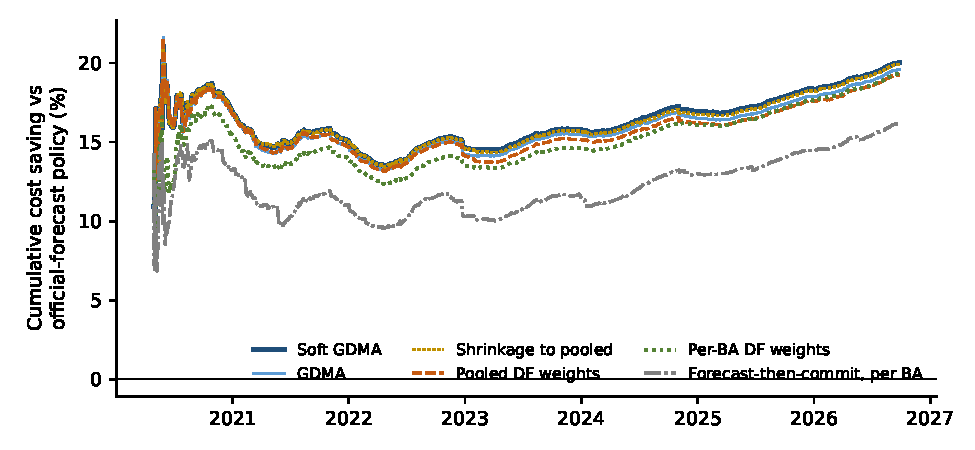
\includegraphics[width=\textwidth]{figures/cumulative.pdf}
\caption{Cumulative system-wide cost saving relative to the official-forecast policy ($W=28$).}\label{fig:cum}
\end{figure}

\subsection{Segments}

\begin{figure}[t]
\centering
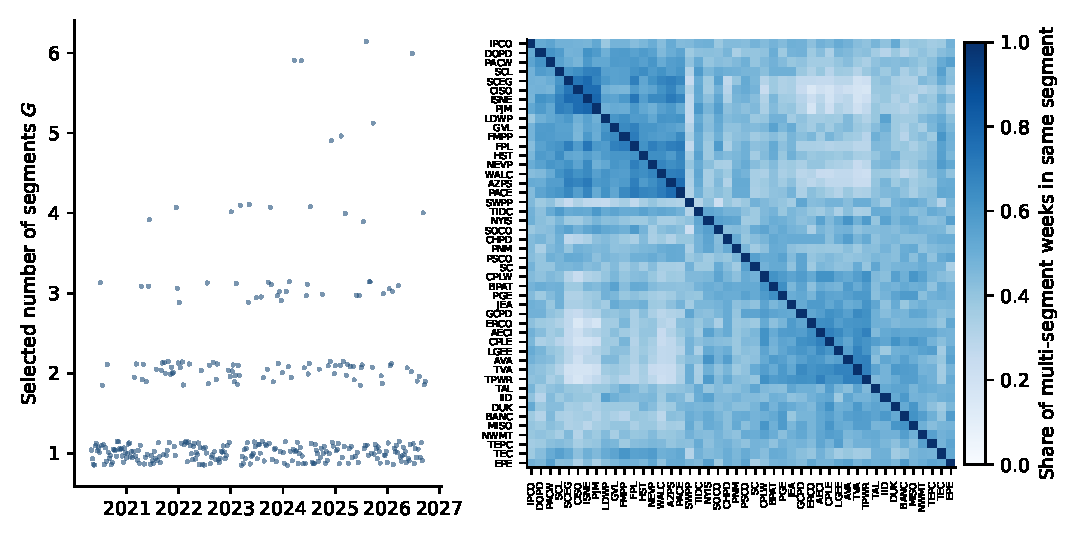
\includegraphics[width=\textwidth]{figures/segments.pdf}
\caption{Left: number of segments selected by GDMA in each weekly re-estimation ($W=28$). Right: among the weeks with $G\ge2$, share of weeks in which two BAs belong to the same segment, ordered by average-linkage clustering.}\label{fig:segments}
\end{figure}

GDMA uses one segment in about two thirds of the weeks and two or more in the rest; multi-segment weeks occur in every year from 2021 onwards (Figure~\ref{fig:segments}, left).
The co-membership matrix (right) reveals two stable segments.
The first contains 17 BAs, among them PJM, CAISO, ISO New England, Florida Power \& Light, Arizona Public Service, Nevada Power and both PacifiCorp areas; their combinations rely almost entirely on the learned models (weights of 0.38 on the hourly regression and 0.47 on LightGBM) and put only 0.12 directly on the official forecast.
The second contains 28 BAs, including MISO, ERCOT, the Southern Company, NYISO, TVA, Bonneville and Duke Energy, and puts 0.39 directly on the official forecast.
Southwest Power Pool often forms a segment of its own.
The two main segments have the same average critical ratio (0.874 and 0.873), so the segmentation is not a relabelling of cost asymmetries; nor does it follow geography or market design, since both contain ISOs and vertically integrated utilities from the East and the West.
What separates them is how much the operator's own forecast adds to what can be learned from recent demand---information that a central planner cannot read off the organisational chart of the grid, but that GDMA extracts from the data.

\subsection{Extreme events and robustness}\label{sec:robust}

\begin{table}[t]
\centering
\caption{System cost during extreme events relative to the official-forecast policy ($W=28$): Winter Storm Uri (10--20 February 2021), Winter Storm Elliott (22--27 December 2022) and the heat wave of 15 July--15 August 2023.}\label{tab:events}
\small
\begin{tabular}{@{}lccc@{}}
\toprule
Method & Winter Storm Uri (10--20 Feb 2021) & Winter Storm Elliott (22--27 Dec 2022) & Heat wave (15 Jul--15 Aug 2023) \\
\midrule
Official forecast & 1.000 & \textbf{1.000} & 1.000 \\
Equal weights & 1.133 & 2.534 & 1.366 \\
Best single (per BA) & 0.881 & 1.264 & 0.796 \\
Pooled DF weights & \textbf{0.842} & 1.318 & \textbf{0.778} \\
Per-BA DF weights & 0.848 & 1.184 & 0.790 \\
Shrinkage to pooled & 0.845 & 1.210 & 0.779 \\
Two-step $k$-means & \textbf{0.842} & 1.239 & 0.780 \\
Forecast-then-commit, per BA & 0.973 & 1.584 & 0.796 \\
Forecast-then-commit, grouped & 0.946 & 1.481 & 0.785 \\
\textbf{GDMA} & \textbf{0.842} & 1.318 & 0.782 \\
\bottomrule
\end{tabular}
\end{table}

Table~\ref{tab:events} examines three extreme episodes.
During Winter Storm Uri and the 2023 heat wave, the decision-focused combinations cost 15--22\% less than the official-forecast policy, in line with their average performance.
Winter Storm Elliott is different: the sudden cold snap of December 2022 was forecast much better by the operators, whose forecasts use weather information that none of our candidates sees directly, and every combination is 18--32\% more expensive than the official policy over those six days.
Soft GDMA and shrinkage limit the damage better than pooled weights and plain GDMA (1.21 against 1.32), presumably because unit-level shrinkage lets the BAs whose official forecasts are most informative keep more weight on them.
The episode is a reminder that combination weights learned in calm weeks cannot anticipate an abrupt regime change; Section~\ref{sec:global} adds candidates driven by archived deterministic and ensemble weather forecasts and shows that they close more than half of this gap.

\begin{table}[t]
\centering
\caption{Sensitivity to the cost asymmetry ($W=28$): system cost relative to the official-forecast policy when every BA has the same critical ratio $\tau$, and under the calibrated heterogeneous ratios.}\label{tab:tau}
\small
\begin{tabular}{@{}lccccc@{}}
\toprule
Method & $\tau=0.5$ & $\tau=0.8$ & $\tau=0.9$ & $\tau=0.95$ & Calibrated \\
\midrule
Official forecast & 1.0000 & 1.0000 & 1.0000 & 1.0000 & 1.0000 \\
Equal weights & 1.4033 & 1.4353 & 1.4860 & 1.5265 & 1.5287 \\
Best single (per BA) & 0.8158 & 0.7921 & 0.8081 & 0.8326 & 0.8245 \\
Pooled DF weights & 0.7988 & 0.7775 & 0.7897 & 0.8136 & 0.8075 \\
Per-BA DF weights & 0.8007 & 0.7798 & 0.7914 & 0.8140 & 0.8069 \\
Shrinkage to pooled & 0.7932 & \textbf{0.7714} & 0.7834 & 0.8067 & 0.8009 \\
Two-step $k$-means & 0.7950 & 0.7736 & 0.7857 & 0.8101 & 0.8041 \\
Forecast-then-commit, per BA & 0.8136 & 0.7944 & 0.8144 & 0.8483 & 0.8382 \\
Forecast-then-commit, grouped & 0.8128 & 0.7916 & 0.8066 & 0.8337 & 0.8260 \\
GDMA & 0.7968 & 0.7750 & 0.7868 & 0.8094 & 0.8042 \\
GDMA, minimum hold-out rule & 0.7981 & 0.7762 & 0.7880 & 0.8098 & 0.8032 \\
\textbf{Soft GDMA} & \textbf{0.7931} & 0.7714 & \textbf{0.7832} & \textbf{0.8065} & \textbf{0.7999} \\
\bottomrule
\end{tabular}
\end{table}

Table~\ref{tab:tau} replaces the calibrated critical ratios by a common $\tau$ for every BA, from the symmetric case $\tau=0.5$ to the highly asymmetric $\tau=0.95$.
The level of the savings changes little---soft GDMA saves 19--23\% relative to the official-forecast policy---and so does the ranking: soft GDMA is the cheapest method for $\tau\in\{0.5,0.9,0.95\}$ and under the calibrated ratios, and ties with shrinkage for $\tau=0.8$.
The advantage of decision-focused over forecast-then-commit combination grows with the asymmetry, from 2.5\% at $\tau=0.5$ to 3.4\% at $\tau=0.95$ relative to the better forecast-then-commit method, as expected: the more asymmetric the cost, the more the best combination for the decision departs from the most accurate one.
